%%%%%%%%%%%%%%%%%%%%%%%%%%%%%%  IEEEsample.tex
%%%%%%%%%%%%%%%%%%%%%%%%%%%%%%%%%%%%%%%%%
%%%%%%%%%%%%%%%%%%%%%%%    More information: see the header of IEEEtran.sty
%%%%%%%%%%%%%%%%%%%%%%%
%%%%%%%%%%%%%%%%%%%%%%%%%%%%%%%%%%%%%%%%%%%%%%%%%%%%%%%%%%%%%%%%%%%%%%%%%%%%%%%%
%%%%

\documentclass[11pt,twoside, onecolumn]{IEEEtran}
%\documentclass[conference]{IEEEtran}

%%%\IEEEoverridecommandlockouts

\usepackage[ruled]{./algorithm2e}
%%for algorithm2e package, label has to be following caption in the same line!!!
\renewcommand{\algorithmcfname}{ALGORITHM}
\SetAlFnt{\small}
\SetAlCapFnt{\small}
\SetAlCapNameFnt{\small}
\SetAlCapHSkip{0pt}
\IncMargin{-\parindent}



%% \RequirePackage{times}
%% \RequirePackage{algorithmic}
%% \PassOptionsToPackage{boxed}{algorithm}
%% \RequirePackage{algorithm}
%% \RequirePackage{multicol}
%\renewcommand{\algorithmicrequire}{\textbf{Inputs:}}
%\renewcommand{\algorithmicensure}{\textbf{Outputs:}}
%\DeclareMathAlphabet{\mathtsl}{OT1}{ptm}{m}{sl}

%\def\BibTeX{{\rm B\kern-.05em{\sc i\kern-.025em b}\kern-.08em1
%    T\kern-.1667em\lower.7ex\hbox{E}\kern-.125emX}}

%\newtheorem{theorem}{Theorem}
%\newtheorem{lemma}{Lemma}
%\newtheorem{example}{Example}
%\newtheorem{corollary}{Corollary}

\RequirePackage{amssymb, mathptm}
\usepackage{amsbsy}
\usepackage{graphicx}
\usepackage{helvet}
\usepackage{enumerate}
\usepackage{amsmath}
\usepackage{amsfonts}
\usepackage{graphicx}
\usepackage{multirow}
\usepackage{subfig}
\usepackage{comment}



%%indent in algorithm


%\setcounter{page}{1}


% New command for the table notes.
\def\tabnote#1{{\small{#1}}}

% New command for the line spacing.
\newcommand{\ls}[1]
    {\dimen0=\fontdimen6\the\font
     \lineskip=#1\dimen0
     \advance\lineskip.5\fontdimen5\the\font
     \advance\lineskip-\dimen0
     \lineskiplimit=.9\lineskip
     \baselineskip=\lineskip
     \advance\baselineskip\dimen0
     \normallineskip\lineskip
     \normallineskiplimit\lineskiplimit
     \normalbaselineskip\baselineskip
     \ignorespaces
    }
%\renewcommand{\algorithmicrequire}{\textbf{Input:}}
%\renewcommand{\algorithmicensure}{\textbf{Output:}}

\newcommand{\beq}{\begin{equation}}
\newcommand{\eeq}{\end{equation}}
\newcommand{\beqarr}{\begin{eqnarray}}
\newcommand{\eeqarr}{\end{eqnarray}}
%\newcommand{\ov}{\overline}
\newcommand{\ov}{\bar}
\newcommand{\xor}{\bigoplus}
\newcommand{\Fm}{{\mathbb{F}}}



%the following is for space before and after align or other equation environment.

%%
\newtheorem{Algorithm}{Algorithm}[section]
\newtheorem{Definition}{Definition}[section]
\newtheorem{Example}{Example}[section]
\newtheorem{Proposition}{Proposition}[section]
\newtheorem{Lemma}{Lemma}[section]
\newtheorem{Theorem}{Theorem}[section]
\newtheorem{Corollary}{Corollary}[section]
\newtheorem{Conjecture}{Conjecture}[section]
\newtheorem{Problem}{Problem}[section]
\newtheorem{Notation}{Notation}[section]
\newtheorem{Setup}{Problem Setup}[section]
%%%

%%set spacing between table columns
\setlength{\tabcolsep}{3pt}

\begin{document}

%\thispagestyle{empty}
%\pagestyle{empty}

\ls{1.1}

\title{\large{\textsc{Report  on Algorithmic Complexity Analysis in Design Automation and Formal Verification}}}
\author{Xiaojun Sun\\
A Technical Report\\
in partial fulfillment of requirements for PhD qualification\\
of Computer Engineering Program, University of Utah\\
Fall Semester 2013
}

%%\author{\IEEEauthorblockN{Jinpeng Lv and Priyank Kalla}\thanks{This work is sponsored in part by a grant from NSF \#CCF-546859.}
%\IEEEauthorblockA{Department of  Electrical and Computer Eng.\\
% University of Utah, Salt Lake City, UT-84112 \vspace{-0.3in}
 %\{lv, kalla\}@eng.utah.edu
% }
%\and
%\IEEEauthorblockN{Florian Enescu} \thanks{\normalsize  978-3-9810801-8-6/DATE12/$\copyright 2012$ EDAA}
%\IEEEauthorblockA{Department of Mathematics and Statistics\\
% Georgia State University,  Atlanta, GA 30302-4038 \vspace{-0.3in}
% fenescu@mathstat.gsu.edu
%} 
%
 
\maketitle

%\markboth{MS Proposal by Tim Pruss}{}
\newcommand{\Fq}{{\mathbb{F}}_{q}}
\newcommand{\Fkk}{{\mathbb{F}}_{2^k}}
\newcommand{\Fkkx}[1][x]{\ensuremath{\mathbb{F}}_{2^k}[#1]\xspace}
\newcommand{\Grobner}{Gr\"{o}bner\xspace}
\newcommand{\B}{{\mathbb{B}}}
\newcommand{\Z}{{\mathbb{Z}}}
\newcommand{\F}{{\mathcal{F}}}
\newcommand{\G}{{\mathcal{G}}}
\newcommand{\R}{\mathbb{R}}
%%%

\newcommand{\debug}[1]{\textcolor{gray}{[ #1 ]}}


%\thispagestyle{empty}

%%%%%%%%%%%%%%%%%%%% Include your files here %%%%%%%%%%%%%%%%%%%%%
\section{Linear Complexity}
\subsection{Definition}
Computational complexity notions strictly defined in [1] are preliminaries to this report.
\begin{Definition}
Computational complexity $\Theta(n)$ is defined as \emph{linear complexity}. The property of
linear complexity algorithm is the time or space cost of this algorithm is a linear function
of input data size $n$.
\end{Definition}

The following algorithm is a simple example of linear complexity algorithm on both time
and space consumption.
\begin{Example}
An array with $n$ integers is stored within a 1-dimension linked list. A traversal algorithm
starts from the head of list, transit through the pointer pointing to successor node, stops
when reaching the end node. The space complexity of this linked list is $\Theta(n)$, and
time complexity of traversal algorithm is $\Theta(n)$.
\end{Example}

\subsection{Design Automation Applications}
\label{sec:graph}
Algorithms from graph theory are a big portion of algorithms in design automation because
graph representation is widely adopted in different aspects of electrical engineering. For example,
graph representation covers finite state machine, labeled petri-net, delay network and abstraction
of circuits. If there is a loop in state transition sequence, or feedback loop in gate-level
implementation, there is also a cycle in corresponding graph representation. An efficient
algorithm can check whether there exists a cycle in a directed graph, which is
\emph{Topological Sort}.

In graph theory, a topological sort or topological ordering of a directed acyclic graph (DAG) is a linear
 ordering of its vertices, in which each vertex comes before all vertices to which it has outbound edges. 
 Every DAG has one or more topological sorts.

\begin{algorithm}[hbt]
\SetAlgoNoLine
 \KwIn{A directed graph $G=(V,E)$}
 \KwOut{A list of topological sorted vertices\\} %, a Gr\"{o}bner basis
  Initialize $S$;\\
  $V_0 \gets$ all vertices with no incoming edges;\\
  \While{$V$ is non-empty}{
 	 remove a vertex $v$ from $V_0$;\\
 	 insert $v$ into $S$;\\
 	 \For{each vertex $u$ with an edge $e = <v,u>$}
 	 {
 	 	remove edge $e$ from $G$;\\
 	 	\If{u has no incoming edges}
 	 	{
 	 		insert $u$ into $V_0$;
 	 	}
 	 }
   }
   \If{$G$ still has edges}
   {
   		\Return{ "Graph has cycle(s)"};\\
   		}
   	\Else{
   		\Return $S$;
   		}
\caption{The Topological Sort Algorithm$^{[2]}$}\label{alg:top}
\end{algorithm}

\subsection{Computational Analysis}
According to algorithm \ref{alg:top}, before algorithm terminated every vertex and edge is scanned only once then directly
removed. So in the worst case, there are no edges left in original graph, all vertices and edges are
visited, the time complexity is $\Theta(|V|+|E|)$, linear to number of vertices and edges in graph.

\subsection{Discussion}
Linear complexity algorithm is low-complexity algorithm, the time/space cost grows along with the
size of input (usually given in a limited size). In general an even lower complexity usually means
$O(logn)$ or $O(n^{1/k})$ complexity which is hard to achieve. As to topological sort, when the vertices
and edges in original graph are given arbitrarily, there is no alternative algorithm with lower complexity.

\section{Polynomial Complexity}
\subsection{Definition}
\begin{Definition}
\emph{Polynomial complexity} is denoted by $O(n^d)$, where $d$ is a constant number. The property
of polynomial complexity algorithm is the time and space cost of this algorithm is polynomial function
of input size $n$.
\end{Definition}

Logarithmic complexity is
also polynomial complexity because it satisfies the upper bound when taking $d=1$. Linear complexity belongs
to polynomial complexity since $\Theta(n) = O(n^1)$. If $d=0$, it degenerates to constant complexity $O(1)$.

\begin{Example}
The insert sort of an array has polynomial complexity $O(n^2)$.
\end{Example}

\subsection{Design Automation Applications}
In physical design automation there is a special routing problem for interconnect wires. In PCB layout,
the interconnect wires are usually assigned to different copper layers to avoid crossover; wires within the 
same layer are not allowed for crossover. Since copper on the top layer is easy to be etched, industry
requires designers to put the most complicated pattern on top layer. So top layer of interconnection usually requires
the largest number of wires. This problem can be abstracted as:

%%%%%%%%%%%%%%%%%%%%%%% fig:pcb here!!
\begin{figure}[hbt]
	\begin{center}
	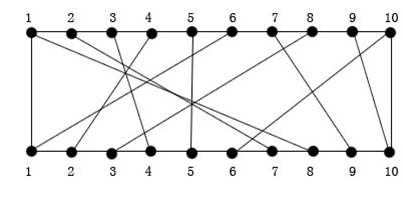
\includegraphics[scale=0.4]{fig_pcb.png}
	\end{center}
	\caption{Example bipartite graph of PCB routing problem[10]}
	\label{fig:pcb}
\end{figure}

Given a bipartition graph, there exists an edge for a pair between 2 sets: $(i,\pi(i))$, $\pi(i)$
is a permutation of $\{1,2,\dots,n\}$. 
$\forall 1\leq i < j\leq n$, edge $(i,\pi(i))$ has crossover with edge $(j,\pi(j))$ if and only if
$\pi(i) > \pi(j)$.
Find the maximal subset of these edges with no crossover. In fig.\ref{fig:pcb}, the desired \emph{maximal no-crossover subset} (MNS) is $\{(4,2),(5,5),(7,9),(9,10)\}$.

This problem has a solution based on a polynomial complexity algorithm. The main idea of that algorithm
is \emph{dynamic programming} (DP).

Denote a part of wires by set $N(i,j) = \{t | (t, \pi(t)) \in Nets, t \leq i, \pi(t) \leq j \}$, its
MNS is denoted by $MNS(i,j)$, its size $|MNS(i,j)| = Size(i,j)$. Then it follows deduction equations:
\begin{equation}
 Size(1,j) = \left\{
\begin{array}{lcl}
0       &      & {j < \pi(1)}\\
1     &      & {j \geq \pi(1)}
\end{array} \right. 
\end{equation}
\begin{equation}
 Size(i,j)\ \ (i>1) = \left\{
\begin{array}{lcl}
Size(i-1,j)       &      & {j < \pi(i)}\\
max\{Size(i-1,j), Size(i-1,\pi(i)-1)+1\}     &      & {j \geq \pi(i)}
\end{array} \right. 
\end{equation}
Equation (1) is the initial value of $Size(i,j)$ when $i=1$, it is deduced with $j$ increasing, MNS size equals to 0 until $j$ reaches the position defining first edge. Equation (2) means every time the algorithm
sweeping $j$ to define a new edge, it is necessary to compare the new size including this edge or not.

Pseudo codes are easy to get from deduction equations for dynamic programming problems. 
\subsection{Computational Analysis}
From the deduction equations, this dynamic programming algorithm will fill up a matrix when getting
answer to the problem, and each entry in the matrix will be updated only once, so both time complexity
and space complexity for this DP algorithm is $O(n^2)$, a polynomial complexity.

\subsection{Discussion}
\label{sec:LIS}
An alternative algorithm for this problem lowers down the time complexity.
By observing optimal solution to MNS problem, the equivalent problem is to find a Longest Increasing
Subsequence (LIS) in permutation $\{\pi(1),\pi(2),\dots,\pi(n)\}$. Fortunately there is a $O(nlogk)$
algorithm to compute LIS. 

The thought of algorithm is: use a stack to maintain a current longest sequence. Scan the whole array,
compare the top of stack with current element $temp$. If $temp$ is larger than stack top, push it in
stack so that current LIS is extended. Otherwise, binary-search the first element larger than $temp$
in the stack, then replace it with $temp$. At last the size of stack is the length of LIS.

For example, given sequence $1,5,8,3,6,7$. The stack is $1,5,8$, when reading 3, search and find 5 in
stack, replace with 3 to get 1,3,8; then read in 6, replace 8 in stack again; at last read in 7. The
final stack is 1,3,6,7.

This improved algorithm uses a loop to scan the array, then use binary search to find desired replacing
elements. Assume the length of LIS is $k$, then in the worst case every time a binary search is required
in $k$ length subsequence, the time complexity is $O(nlogk)$. The result given by this algorithm is
guaranteed to be optimum, so it is not heuristic. 

\section{Exponential Complexity}
\subsection{Definition}
\begin{Definition}
\emph{Exponential complexity} is complexity $O(r^n)$, where $r$ is a constant number. Exponential complexity
algorithm has the property that time/space cost is exponential function of problem size $n$.
\end{Definition}

Exponential complexity is not a polynomial complexity. Usually it indicates the time/space cost explodes
with input size increasing; an algorithm with exponential complexity is common in brute-force techniques
and not considered as an efficient and optimal choice in general case.

\subsection{Formal Verification Applications}
\label{sec:3sat}
Circuit satisfiability (SAT) problem is a typical problem which has no polynomial complexity algorithm
to find optimal solution. For example, given a circuit with primary inputs $\{a,b,c\}$, the output
$Y = (a \land b) \lor \bar{c}$. SAT problem is: is there any boolean vector assignment to primary inputs
so that $Y = 1$?

%%%%%%%%%%%%% fig:SAT here !!!
\begin{figure}[hbt]
	\begin{center}
	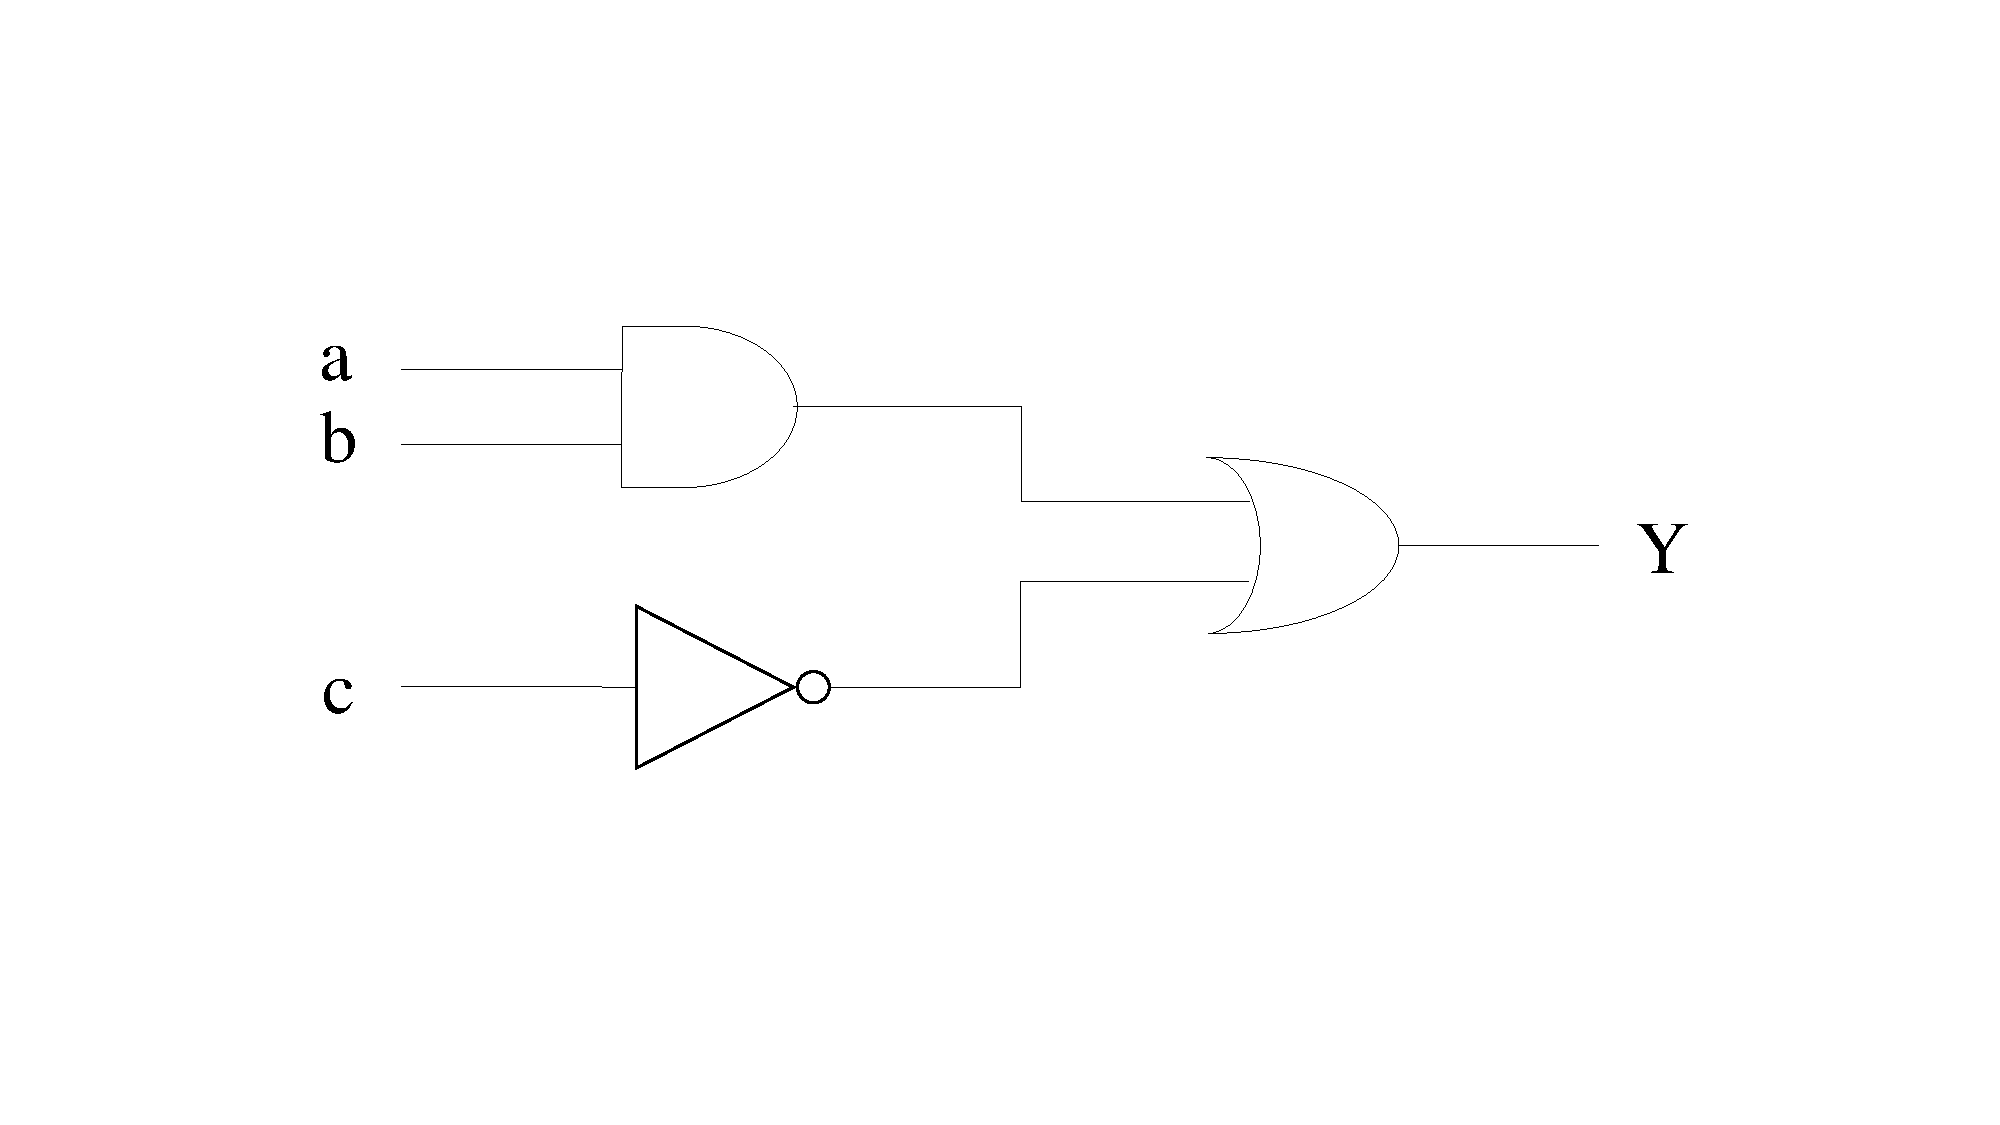
\includegraphics[scale=0.4]{fig_SAT.pdf}
	\end{center}
	\caption{Sample circuit for SAT problem}
	\label{fig:SAT}
\end{figure}

Following the boolean logic, any boolean description of SAT problem can be written in conjunctive
normal form (CNF). If the number of literals in every clause of CNF expression is limited to 3, 
the SAT problem degenerates to 3-SAT problem. The naive method to solve this problem is to scan
all possible assignments on inputs to check 3-SAT. In worst case, if a circuit has $n$ primary
inputs, every input could be assigned $\{0,1\}$, the exhaustive checking algorithm cost $2^n$ checks,
the time complexity is $O(2^n)$, this is an exponential complexity.

\subsection{Discussion}
According to literature search, currently no polynomial lower bound has been proved for 3-SAT problems,
which means there is no algorithm can provide a polynomial complexity in worst case.
However, some refinements are effective to lower down time cost in practice.
One algorithm improves time complexity to $O(r^n), r < 2$.
\begin{algorithm}[hbt]
\SetAlgoNoLine
 \KwIn{A CNF expression with at most 3 literals in a clause}
 \KwOut{An legal assignment of input satisfies given CNF or claim no available assignments\\} %, a Gr\"{o}bner basis
  Check whether current assignment satisfies, if yes return current assignment;\\
  \While{pick arbitrary clause $C = \alpha_1 \lor \alpha_2 \lor \alpha_3$ that still unsatisfied}{
 	 set $\alpha_1$ to "true", reduce original CNF and recursively check rest clauses;\\
 	 set $\alpha_1$ to "false" and $\alpha_2$ to "true", reduce original CNF and recursively check rest clauses;\\
 	 set both $\alpha_1$ and $\alpha_2$ to "false" and assign "true" to $\alpha_3$, reduce original CNF and recursively check rest clauses;\\
 }
 \If{Cannot find any assignment to satisfy original CNF}
 {
 \Return{"No satisfiable assignments"}
 }
 	 \caption{The Refined Exponential Time 3-SAT Algorithm$^{[2]}$}\label{alg:3sat}
\end{algorithm}
\begin{Theorem}
Algorithm \ref{alg:3sat} solves 3-SAT problem with time complexity $O(1.8393^n)$.
\end{Theorem}

\textit{Proof}[10]\ \ \ Correctness: assignment returned by the algorithm satisfies original CNF expression.
When the algorithm claims "no satisfiable assignments", for all clauses in form
$C = \alpha_1 \lor \alpha_2 \lor \alpha_3$, following possible assignments are checked:\par
(1) $\alpha_1 = TRUE$;\par
(2) $\alpha_1 = FALSE$ and $\alpha_2 = TRUE$;\par
(3) $\alpha_1 = \alpha_2 = FALSE$ and $\alpha_3 = TRUE$.\\
Any assignments must belong to one and only one kind of above 3 situations. Since the while loop
will not terminate unless all clauses are recursively checked, at this time there is no assignment
making original CNF expression be true. 

Complexity: Assume $T(n)$ is the time algorithm operates on CNF containing $n$ literals in total.
Let $m$ be the number of clauses in this CNF expression, then $m = O(n^3)$ since every clause
has at most $3$ literals. In each situation of recursion, the size of original problem is
scaled down to $(n-1), (n-2), (n-3)$ after determining assignments for $\alpha_1,(\alpha_1,\alpha_2),(\alpha_1,\alpha_2,\alpha_3)$. Reducing procedure scans $m$ clauses and justifying satisfaction requires 
scan all $n$ literals to take their values. So deduction equation on runtime is
$$T(n) \leq T(n-1) + T(n-2) + T(n-3) + O(n+m)$$
Solution is $T(n) = O(1.8393^n)$, while $1.8393$ is the largest root of equation $x^3 = x^2 + x + 1$. \ \ \ \ \ \ \ \ \ \ \ \ \ \ \ \ \ \ \ \ \ \ \ $\Box$

\section{NP-Complete}
\subsection{Definition}
\begin{Definition}
A decision problem belongs to $P$ when there is a polynomial time complexity solution.
\end{Definition}

Decision problem is a kind of problems can be answered by $"YES"$ or $"No"$. For example, the LIS problem
mentioned in \ref{sec:LIS} can be classified to $P$ if it is asked in this form: "Does there exist a $LIS$ of
length $k$?". The LIS algorithm also gives the subsequence when solving this decision problem.

\begin{Definition}
Nondeterministic polynomial problems ($NP$) is a class of decision problems, when given a testcase,
the problem can verify the testcase within polynomial complexity time.
\end{Definition}

A set of assignments can be verified in 3-SAT problem within polynomial time, and 3-SAT is a decision
problem. So 3-SAT$\in NP$. 

\begin{Definition}
\label{def:nphard}
A problem $\Pi$ is \emph{NP-hard} if and only if, for any problem $\Pi' \in NP$, there is a polynomial-time Turing reduction
from $\Pi'$ to $\Pi$. A Turing reduction means a reduction that can be executed on a Turing machine. Polynomial-time Turing reductions are also called \emph{Cook reductions}.
\end{Definition}

Note that NP-hard problems are not necessarily decision problems. 
According to this definition, a NP-hard problem is not easier than any other NP problems. If a NP-hard
problem is solved in polynomial time, then all $NP$ problems have algorithms to find solutions in polynomial time.

\begin{Definition}
If a problem is NP-hard, and it belongs to NP, then this problem is \emph{NP-Complete}.
\end{Definition}

%%%%%%%%%%%%%%%%% fig:NP here !!!!!!!!!!!!
\begin{figure}[hbt]
	\begin{center}
	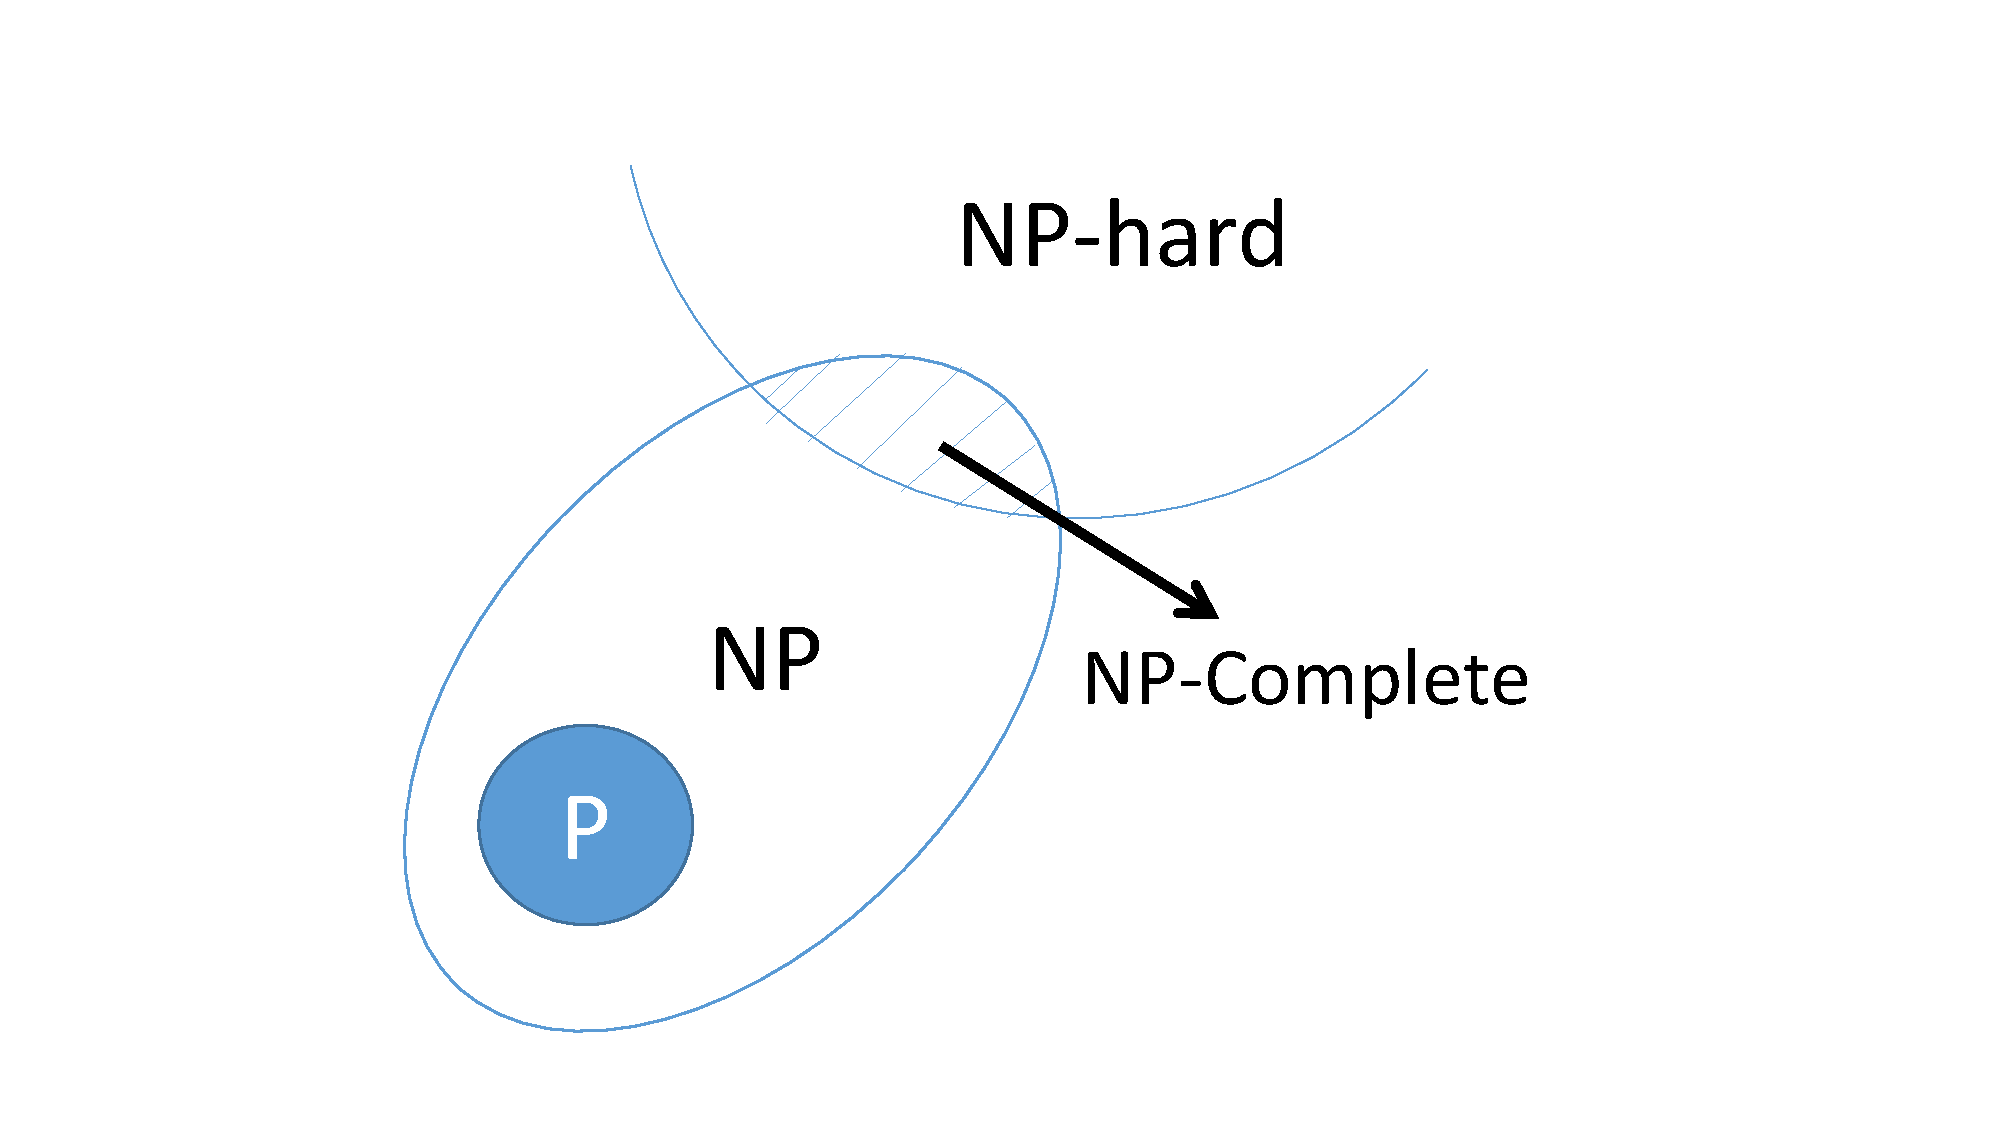
\includegraphics[scale=0.4]{fig_NP.pdf}
	\end{center}
	\caption{A popular graph illustrating relations among P, NP, NP-hard and NP-Complete}
	\label{fig:NP}
\end{figure}

Fig.\ref{fig:NP} illustrates relations between these classes of problems. Note that $P!=NP$ and
$P$ disjoint with $NP$-$hard$ are just conjectures and need to be proved.

To directly prove that a problem is NP-hard or NP-Complete is difficult. Currently most proofs are based
on finding a polynomial time Turing reduction from SAT problem. SAT problem is proved to be NP-Complete in
[4]. If a polynomial time Turing reduction from SAT problem to given problem $\Pi$ is found, then $\Pi$
is not easier than SAT problem. So $\Pi$ is proved to be NP-hard or NP-Complete (if $\Pi \in NP$).

\subsection{Design Automation Applications}
Covering problem is important in logic synthesis. For a circuit with specification set $S = \{s_1, s_2, s_3, s_4\}$, there are 3 possible gate implementations, where $G_1$ satisfies $\{s_1, s_2\}$, $G_2$ satisfies
$\{s_2,s_3\}$ and $G_3$ satisfies $\{s_3,s_4\}$. The question is: is there a set of gate implementations
$\{G_i\}$ that every gate implementation is disjoint with each other on satisfiable specifications, 
and their union equals to $S$? In this example the answer is yes, the a desired solution is $\{G_1, G_3\}$.

This problem is called \emph{exact covering} problem. 
\begin{Theorem}
Exact covering problem (ECP) is NP-Complete.
\end{Theorem}

\textit{Proof} \ \ \ Given a set $\{G_i\}$, this problem can be verified by scanning every element in
$\{G_i\}$ can compare with $S$, this can be done within polynomial time, so $ECP \in NP$.

Following argument proves that there is a polynomial time reduction from ECP to SAT. 

Construction: $n$ is the number of specifications, $m$ is the number of candidate gate implements. Assume a set of
variables $x_1,x_2,\dots,x_n$ and a CNF $F = C_1\land C_2\land \cdots \land C_m$ where clause 
$C_j = z_{j1}\lor z_{j2} \lor \cdots \lor z_{js_j}$, $j = 1,2,\dots,m$; $z$ is literal based on $x$.
Objective is to construct desired subset $W = \{G_i\}$ of finite set $S$ so that $F$ is satisfied
if and only if $W$ contains the exact cover of $S$.
Let $S = \{x_1,x_2,\dots, x_n, C_1, C_2,\dots, C_m\} \bigcup \{p_{jt}\ |\ 1\leq t \leq s_j, 1\leq j\leq m \}$,
where $p_{jt}$ represents literal $z_{jt}$ in $C_j$. For each variable $x_i$, there are 2 subset
$T_i^T$ and $T_i^F$. $T_i^T$ includes variable $x_i$ itself, and all corresponding literals
equal to $\neg x_i$; $T_i^F$ also includes variable $x_i$ itself, with all corresponding literals
equal to $x_i$, i.e.
$$T_i^T = \{x_i, p_{jt}\ |\ z_{jt} = \neg x_i, 1\leq t\leq s_j, 1\leq j\leq m\},$$
$$T_i^T = \{x_i, p_{jt}\ |\ z_{jt} =  x_i, 1\leq t\leq s_j, 1\leq j\leq m\}.$$
Since other subsets do not include $x_i$, any exact cover $U$ must include exactly one
of $T_i^T$ and $T_i^F$. Assign $x_i = 1$ if and only if $U$ contains $T_i^T$, thus assignment
$x_i = 0$ equals to $U$ containing $T_i^F$. Additionally, for each clause $C_j$, it has $s_j$ subsets:
$C_{jt} = \{C_j, p_{jt}\}, 1\leq t \leq s_j$. Besides these subsets, every $p_{jt}$ constructs a unit
subset by itself: $\{p_{jt}\}$.

To conclude, $W$ includes following subsets:\par
(1) $\{p_{jt}\}$ (number: $\sum_{j=1}^{m}s_j$)\par
(2) $T_i^T, T_i^F$ (number: $2\times n$)\par
(3) $C_{jt}$ (number: $\sum_{j=1}^{m}s_j$).\par

Reasoning: To prove $F$ is satisfied
if and only if $W$ contains the exact cover of $S$. 

Assume $U \subseteq W$ is exact cover for $S$. Assign $1$ to $x_i$ if $T_i^T \in U$;
assign $0$ to $x_i$ if $T_i^F \in U$. For all $1\leq j\leq m$, there is exactly one $C_{jt} \in U$.
If $T_i^T \in U$, then $p_{jt}\notin T_i^T$, thus $z_{jt} = x_i$, and $x_i$ is already assigned "1", so
$C_j$ is satisfied. On the other hand if $T_i^F \in U$, then $p_{jt}\notin T_i^F$, thus $z_{jt} = \neg x_i$, 
and $x_i$ is already assigned "0", so $C_j$ is also satisfied. Consider every clause been satisfied,
the corresponding assignment satisfies $F$.

If $F$ is satisfiable, assume an assignment $t$ under which $F$ is true. For each $1\leq i \leq n$,
$t(x_i) = 1$ implies $U$ contains $T_i^T$; $t(x_i) = 0$ implies $U$ contains $T_i^F$. For each
$1\leq j\leq m$, since $t$ satisfies $C_j$, there exists a literal $z_{jt}$ so that $t(z_{jt}) = 1$
and $p_{jt}$ not included by $U$, thus $C_{jt}$ could be inserted into $U$. Until this time,
$U$ already covers all $x_i$ and $C_j$, as well as a part of $p_{jt}$. So after add the uncovered
$p_{jt}$ in forms of unit subset $\{p_{jt}\}$ into $U$, $U$ becomes the exact cover of $S$.

With above arguments, $W$ contains exact cover $U$ (existence of $U$) as long as $F$ is satisfied. If $W$ can be 
constructed within polynomial time, it means the ECP can be reduced to a SAT problem in
polynomial time. The maximal number of literals in $F$ is $mn$, so $|S|\leq n+m+mn$, and
number of subsets in $W$ will not exceed $2n+2mn$ while size of single subset is smaller than $n+1$.
Moreover, the construction method is straightforward and able to finish within polynomial time.
Thus, a polynomial time Turing reduction from ECP to SAT is proved.

In conclusion, $ECP \in NP$ and can be reduced to SAT problem, which is NP-Complete. So ECP is NP-Complete.$\Box$

\subsection{Computational Analysis and Discussion}
A naive algorithm for ECP is to enumerate all subsets from $\{G_i\}$. If there are $n$ gate implementations,
number to enumerate is $2^n$, so the time complexity for naive algorithm is $O(2^n)$, it is not a polynomial
complexity.

ECP is NP-Complete indicates there is currently no polynomial time complexity algorithm to find the
solution. However, there are several heuristics can be applied to minimize search space as much as possible.
One of them is DLX algorithm invented by D.E. Knuth[5].

Assume there is a binary matrix $M$, each row of $M$ can represent a gate implementation $G_i$.
Entry $M(i,j) = 0$ means $G_i$ does not satisfy specification $s_j$, $M(i,j) = 1$ means it does satisfy.
For example, following matrix
\begin{equation}
M = \left(
\begin{array}{lcccccr}
0 & 0 & 1 & 0 & 1 & 1 & 0\\
1 & 0 & 0 & 1 & 0 & 0 & 1\\
0 & 1 & 1 & 0 & 0 & 1 & 0\\
0 & 0 & 0 & 1 & 0 & 1 & 0\\
0 & 1 & 0 & 0 & 0 & 0 & 1\\
0 & 0 & 0 & 1 & 1 & 0 & 1
\end{array}
\right)\nonumber
\end{equation}
row 1,4,5 is an exact cover of specification set, because by merging these rows (do XOR for corresponding
entries) the result is a row with all "1" on every column.

\begin{algorithm}[hbt]
\SetAlgoNoLine
 \KwIn{Matrix to be covered $M$}
 \KwOut{A list of row numbers as solution\\} %, a Gr\"{o}bner basis
  \If{Matrix $M$ is empty}
  {
  		\Return{List of solution};
  	}
  Otherwise choose a column $c$; \ \ \ /* deterministically, usually choose the one with least number of "1" entries */\\
  Choose a row $r$ such that $M(r,c) = 1$; \ \ \ /* nondeterministically */ \\
  Add row $r$ to solution list;\\
  \For{each column $j$ such that $M(r,j) = 1$}{
 	 \For{each row $i$ such that $M(i,j) = 1$}
 	 {
 	 	delete row $i$ from $M$;
 	 }
 	 delete column $j$ from $M$;
   }
   Recursively repeat on reduced Matrix;
\caption{Knuth's DLX Algorithm for ECP$^{[5]}$}\label{alg:knuth}
\end{algorithm}

The upper bound of this algorithm is still exponential time complexity. However in experiment,
the search tree usually get very sparse after a few recursions. In general situation, this algorithm
is an efficient heuristic (nondeterministically branch-and-bound) algorithm.

\section{NP-hard}
\subsection{Definition}
The definition of NP-hard problem is stated in DEF. \ref{def:nphard}. In practice, most NP-hard problems
are problems proved no easier than NP-Complete problems but not decision problems.

\subsection{Design Automation Applications} 
A problem related to route among pins is important in design automation.
In fig.\ref{fig:MST}(a), there are 4 pins and routing is only allowed along the grids.
The problem is to find a path of routing to connect all pins with lowest cost on total length of
wires. This problem is called minimal Rectilinear Steiner tree problem (MRST), highly similar to 
minimal Steiner tree problem, which is proved to be NP-hard[7]. Since MRST problem is not a 
decision problem ($\notin NP$), it is NP-hard rather than NP-Complete.

\subsection{Computational Analysis}
There is no polynomial time complexity algorithm to find an optimal solution to this problem.
In order to lower down the time complexity, some heuristics are adopted to approximate the 
optimal solution. One algorithm is to use minimal spanning tree (MST) to approximate MRST,
and the distortion is bounded to a small value.

\begin{Theorem}
The relationship between MST and MRST is:
$$\frac{Cost(MST)}{Cost(MRST)} \leq \frac{3}{2}$$
\end{Theorem}

This assertion is proved by K. Hwang[8], it shows MST algorithm provides a $3/2$-approximation of
MRST problem. MST has deterministic algorithm such as Prim's Algorithm and Kruskal's Algorithm,
both have polynomial time complexity $O(|E|log|V|)$. Considering $|V|$ is the number of pins $n$,
and $|E|$ is the number of edges connect every pair of pins ($n(n-1)/2$), the complexity is
written as $O(n^2logn)$.

\subsection{Discussion}
It is hard to find even lower complexity algorithm than MST heuristic. However, the quality
of solution given by MST approximation is relatively low (compare fig.\ref{fig:MST}(b) to fig.\ref{fig:Steiner}(b)).

\begin{figure}[hbt]
	\begin{center}
	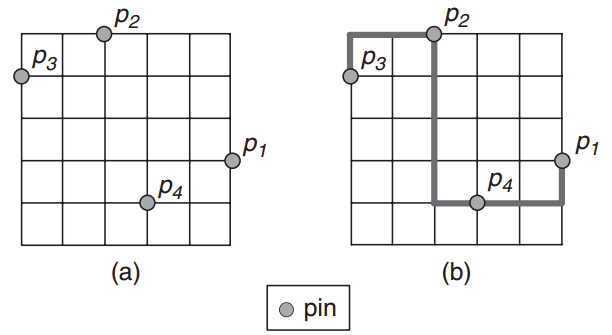
\includegraphics[scale=0.4]{MST.png}
	\end{center}
	\caption{Example of MST heuristic[9]}
	\label{fig:MST}
\end{figure}

\begin{figure}[hbt]
	\begin{center}
	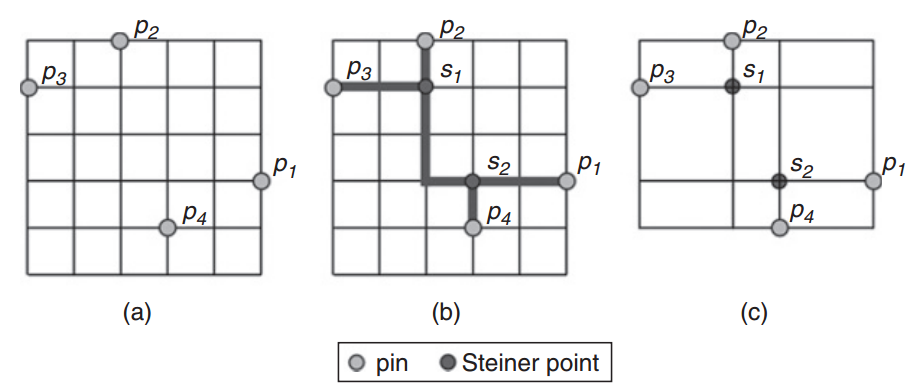
\includegraphics[scale=0.4]{Steiner.png}
	\end{center}
	\caption{Example of optimal routing with Steiner points [9]}
	\label{fig:Steiner}
\end{figure}

The iterated 1-Steiner heuristic is applied to improve the quality. 
\begin{algorithm}[hbt]
\SetAlgoNoLine
 \KwIn{A set of $n$ pins $P$}
 \KwOut{A Steiner tree on $P$\\} %, a Gr\"{o}bner basis
  \While{There are places on grids to insert Steiner points}
  {
  	Find a 1-Steiner point which brings maximal improvement on cost by constructing MST with it;\\
  	Add this Steiner point into recording list $S$;\\
  	In refined MST, find existing Steiner points with degree $\leq 2$, remove them from $MST$ and $S$;
  }
  \Return{MST generated by $P \cup S$}
\caption{Iterated 1-Steiner Heuristic Algorithm$^{[6]}$}\label{alg:iter}
\end{algorithm}

In this heuristic, in preparation stage, an ordering of potential Steiner point candidates is calculated by checking the improvement on total
cost of MST generated by $P \cup \{x\}$, $x$ is a candidate. Then the best $n$ candidates are kept,
so the number of iterations are limited to $n$. During each iteration, the removal and MST re-generation
cost $O(n^2logn)$ time. So total time complexity is $O(n^3logn)$, higher than the MST heuristic.
Fig.\ref{fig:iter}(b)-(e) depicts all iterations of this algorithm ($n=4$).

\begin{figure}[hbt]
	\begin{center}
	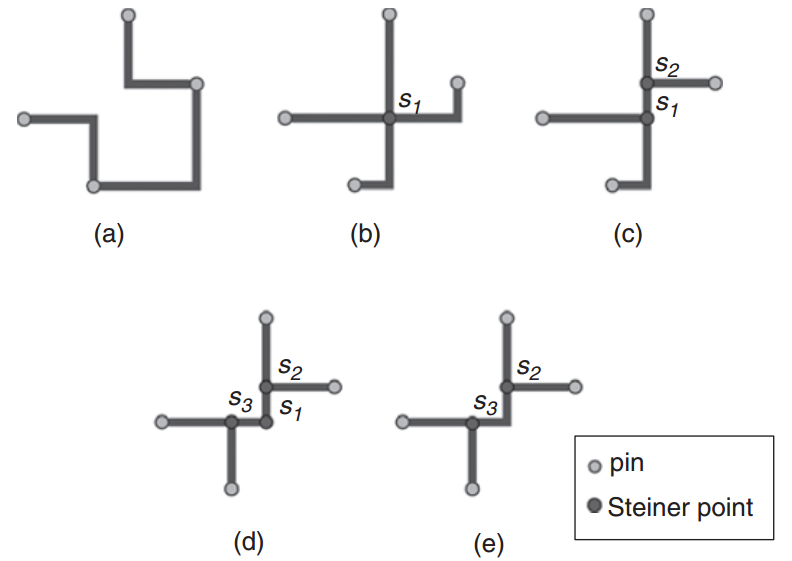
\includegraphics[scale=0.4]{iter.png}
	\end{center}
	\caption{Example of iterated 1-Steiner heuristic algorithm[9]}
	\label{fig:iter}
\end{figure}

Although executed with a higher time complexity, the quality of the solution given by this algorithm is 
greatly improved comparing to MST heuristic. In experiment, this algorithm gives optimal solution for
$n\leq 4$; for $n=5$ which MST heuristic may give a $3/2$ approximation, the iterated 1-Steiner heuristic
gives a tighter $7/6$ approximation in worst case.

%%%%%%%%%%%%%%%%%%%% The bibliography %%%%%%%%%%%%%%%%%%%%%%%%%%%%
\begin{thebibliography}{1}

\bibitem{ref1}
Web lecture from MIT, \emph{Big O Notation}. http://web.mit.edu/16.070/www/lecture/big\_o.pdf

\bibitem{ref2}
Kleinberg J, Tardos E. \emph{Algorithm design}[M]. Pearson Education India, 2006.

\bibitem{ref3}
Jeff Erickson, \emph{"Algorithms course materials"}.

\bibitem{ref4}
Stephen A. Cook (1971). \emph{The Complexity of Theorem-Proving Procedures}. Proc. 3rd Ann. Symp. on Theory of Computer. pp151-158.

\bibitem{ref5}
Knuth D E. \emph{Dancing links}[J]. arXiv preprint cs/0011047, 2000.

\bibitem{ref6}

Kahng, Andrew, and Gabriel Robins. \emph{A new class of Steiner tree heuristics with good performance: the iterated 1-Steiner approach.}  International Conference on Computer-Aided Design,. IEEE, 1990.

\bibitem{ref7}

Richard M. Karp. \emph{Reducibility Among Combinatorial Problems}. In R. E. Miller and J. W. Thatcher (editors). \emph{Complexity of Computer Computations}. New York: Plenum. pp. 85-103.

\bibitem{ref8}

Hwang, Frank K. \emph{On Steiner minimal trees with rectilinear distance.} SIAM journal on Applied Mathematics 30.1 (1976): 104-114.

\bibitem{ref9}

L. Wang, Y. Chang, K. Cheng , Electronic design automation: synthesis, verification, and test[M]. Elsevier, 2009.

\bibitem{ref10}

W. Qu, T. Liu et al., \emph{Algorithm Design and Analysis}. Tsinghua University, 2011

\end{thebibliography}

\end{document}

%%%%%%%%%%%%%%%%%%%%%%%%%%%  End of IEEEsample.tex  %%%%%%%%%%%%%%%%%%%%%%%%%%%